\documentclass{article} % A4 paper and 11pt font size
\setcounter{secnumdepth}{0}

\usepackage{amssymb, amsmath, amsfonts}
\usepackage{moreverb}
\usepackage{graphicx}
\usepackage{enumerate}
\usepackage{graphics}
\usepackage[margin=1.25in]{geometry}
\usepackage{color}
\usepackage{tocloft}
\renewcommand{\cftsecleader}{\cftdotfill{\cftdotsep}}
\usepackage{array}
\usepackage{float}
\usepackage{hyperref}
\usepackage{textcomp}
\usepackage[makeroom]{cancel}
\usepackage{bbold}
\usepackage{alltt}
\usepackage{physics}
\usepackage{mathtools}
\usepackage[normalem]{ulem}
\usepackage{amsthm}
\usepackage{tikz}
\usetikzlibrary{positioning}
\usetikzlibrary{arrows}
\usepackage{pgfplots}
\usepackage{bigints}
\allowdisplaybreaks
\pgfplotsset{compat=1.12}

\theoremstyle{plain}
\newtheorem*{theorem*}{Theorem}
\newtheorem{theorem}{Theorem}
\newtheorem*{lemma*}{Lemma}
\newtheorem{lemma}{Lemma}

\makeatletter
\newcommand{\BIGG}{\bBigg@{3}}
\newcommand{\vast}{\bBigg@{4}}
\newcommand{\Vast}{\bBigg@{5}}
\makeatother

\newenvironment{definition}[1][Definition]{\begin{trivlist}
\item[\hskip \labelsep {\bfseries #1}]}{\end{trivlist}}

\newcommand{\E}{\varepsilon}
\def\Rl{\mathbb{R}}
\def\Cx{\mathbb{C}}

\newcommand{\Ei}{\text{Ei}}

\usepackage[T1]{fontenc} % Use 8-bit encoding that has 256 glyphs
\usepackage{fourier} % Use the Adobe Utopia font for the document - comment this line to return to the LaTeX default
\usepackage[english]{babel} % English language/hyphenation

\usepackage{sectsty} % Allows customizing section commands
\allsectionsfont{\centering \normalfont\scshape} % Make all sections centered, the default font and small caps

\usepackage{fancyhdr} % Custom headers and footers
\pagestyle{fancy} % Makes all pages in the document conform to the custom headers and footers
\fancyhead[L]{\bf Sam Fleischer}
\fancyhead[C]{\bf UC Davis \\ Big Data (MAT280)} % No page header - if you want one, create it in the same way as the footers below
\fancyhead[R]{\bf Spring 2016}

\fancyfoot[L]{\bf } % Empty left footer
\fancyfoot[C]{\bf \thepage} % Empty center footer
\fancyfoot[R]{\bf } % Page numbering for right footer
\renewcommand{\headrulewidth}{0pt} % Remove header underlines
\renewcommand{\footrulewidth}{0pt} % Remove footer underlines
\setlength{\headheight}{25pt} % Customize the height of the header

\newcommand{\VEC}[2]{\left\langle #1, #2 \right\rangle}
\newcommand{\ran}{\text{\rm ran }}
\newcommand{\Hilb}{\mathcal{H}}
\newcommand{\lap}{\Delta}

\newcommand{\littleo}[1]{\text{\scriptsize$\mathcal{O}$}\qty(#1)}

\DeclareMathOperator*{\esssup}{\text{ess~sup}}

\newcommand{\problem}[2]{
\vspace{.375cm}
\boxed{\begin{minipage}{\textwidth}
    \section{\bf #1}
    #2
\end{minipage}}
}

\numberwithin{equation}{section} % Number equations within sections (i.e. 1.1, 1.2, 2.1, 2.2 instead of 1, 2, 3, 4)
\numberwithin{figure}{section} % Number figures within sections (i.e. 1.1, 1.2, 2.1, 2.2 instead of 1, 2, 3, 4)
\numberwithin{table}{section} % Number tables within sections (i.e. 1.1, 1.2, 2.1, 2.2 instead of 1, 2, 3, 4)

\setlength\parindent{0pt} % Removes all indentation from paragraphs - comment this line for an assignment with lots of text

\newcommand{\horrule}[1]{\rule{\linewidth}{#1}} % Create horizontal rule command with 1 argument of height

\usepackage{xcolor}
\definecolor{light-gray}{gray}{0.9}

\title{ 
\normalfont \normalsize 
\textsc{UC Davis, Big Data (MAT280), Spring 2016} \\ [25pt] % Your university, school and/or department name(s)
\horrule{2pt} \\[0.4cm] % Thin top horizontal rule
\Huge Homework \#2 \\ % The assignment title
\horrule{2pt} \\[0.5cm] % Thick bottom horizontal rule
}

\author{\huge Sam Fleischer} % Your name

\date{May 2, 2016} % Today's date or a custom date

\begin{document}\thispagestyle{empty}

\maketitle % Print the title

\makeatletter
\@starttoc{toc}
\makeatother

\pagebreak

%%%%%%%%%%%%%%%%%%%%%%%%%%%%%%%%%%%%%%
\problem{Problem 1}{Let $i = \sqrt{-1}$ and set
\begin{align*}
    A = \qty[\begin{array}{ccc}
        i & 0 & -i \\
        0 & i & -i
    \end{array}].
\end{align*}
Using the null space property, show that $\ell_1$-minimization will recover any $1$-sparse vector $x$, given $Ax = y$.}
\begin{proof}
    Given $x = \qty[x_1, x_2, x_3]^T \in \Cx^3$, $Ax = i\qty[x_1 - x_3, x_2 - x_3]^T = 0$ if $x_1 = x_2 = x_3$.  Thus $\text{null} A = \text{span}\qty(\qty[1,1,1]^T)$.  Let $h \in \text{null} A$.  Then $h = \qty[a, a, a]^T$ for some $a \in \Cx$.  Then choose $S_i = \{i\}$ for $i = 1, 2, 3$.  Then
    \begin{align*}
        h_{S_1} = \qty[\begin{array}{c} a\\0\\0\end{array}], \qquad h_{S_2} = \qty[\begin{array}{c} 0\\a\\0\end{array}], \qquad \text{and} \qquad h_{S_3} = \qty[\begin{array}{c} 0\\0\\a \end{array}]
    \end{align*}
    which gives
    \begin{align*}
        h_{S_1^C} = \qty[\begin{array}{c} 0\\a\\a \end{array}], \qquad h_{S_2^C} = \qty[\begin{array}{c} a\\0\\a \end{array}], \qquad \text{and} \qquad h_{S_3^C} = \qty[\begin{array}{c} a\\a\\0 \end{array}]
    \end{align*}
    Clearly $\norm{h_{S_i}}_1 = \abs{a}$ and $\norm{h_{S_i^C}}_1 = 2\abs{a}$ for $i = 1, 2, 3$.  Thus $\norm{h_S}_1 \leq \norm{h_{S^C}}_1$ for all $h \in \text{null} A$ and all $S \subset \{1,2,3\}$ with $\abs{S} = 1$.  This shows the null space property holds and hence $\ell_1$-minimization will recover any $1$-sparse vector $x$.
\end{proof}
    







%%%%%%%%%%%%%%%%%%%%%%%%%%%%%%%%%%%%%%
\problem{Problem 2}{On the connection between (in)coherence parameter $\mu$ and restricted isometry constant $\delta_s$: Show that $\delta_1 = 0$, $\delta_2 = \mu$, and $\delta_s \leq (s-1)\mu$.}
\begin{proof}
    Let $A \in \Rl^{k \times d}$ where each column is normalized, i.e.~$\norm{A_j}_2 = 1$ for each $j = 1, 2, \dots, d$.  Let $x$ be a $1$-sparse vector of norm $1$, that is, $\abs{x_k} = 1$ for some $k \in \{1, 2, \dots, d\}$ and $x_\ell = 0$ for $\ell \in \{1, 2, \dots, d\}\setminus \{k\}$.  Then $Ax = x_kA_k$, where $A_k$ denotes the $k$\textsuperscript{th} column of $A$.  Since each column is normalized,
    \begin{align*}
        \norm{Ax}_2^2 = \norm{A_j}_2^2 = 1 = \norm{x}_2^2
    \end{align*}
    Since this holds for all $1$-sparse vector, $\delta_1 = 0$.

    Now set $x$ be a $2$-sparse vector of norm $1$, that is $\abs{x_{k_1}}^2 + \abs{x_{k_2}}^2 = 1$ for some $k_1, k_2 \in \{1, 2, \dots, d\}$ and $x_\ell = 0$ for $\ell \in \{1, 2, \dots, d\}\setminus\{x_{k_1}, x_{k_2}\}$.  Then $Ax = x_{k_1}A_{k_1} + x_{k_2}A_{k_2}$.  Thus,
    \begin{align*}
        \norm{Ax}_2^2 = \norm{x_{k_1}A_{k_1} + x_{k_2}A_{k_2}}_2^2 &= \norm{x_{k_1}A_{k_1}}_2^2 + 2\VEC{x_{k_1}A_{k_1}}{x_{k_2}A_{k_2}}_2 + \norm{x_{k_2}A_{k_2}}_2^2 \\
        &= \abs{x_{k_1}}^2\cancelto{1}{\norm{A_{k_1}}_2^2} + 2x_{k_1}x_{k_2}\VEC{A_{k_1}}{A_{k_2}}_2 + \abs{x_{k_2}}^2\cancelto{1}{\norm{A_{k_2}}_2^2} \\
        &= \cancelto{1}{\abs{x_{k_1}}^2 + \abs{x_{k_2}}^2} + 2x_{k_1}x_{k_2}\VEC{A_{k_1}}{A_{k_2}}_2 \\
        &\leq 1 + \VEC{A_{k_1}}{A_{k_2}}_2
    \end{align*}
    since $\displaystyle\max_{\abs{a}^2 + \abs{b}^2 = 1}\qty[ab] = \frac{1}{2}$.  Then since $\abs{\VEC{A_{k_1}}{A_{k_2}}} < \mu$,
    \begin{align*}
        \qty(1 - \mu)\norm{x}_2^2 = 1 - \mu \leq \norm{Ax}_2^2 \leq 1 + \mu = \qty(1 + \mu)\norm{x}_2^2.
    \end{align*}
    Since this holds for all $2$-sparse vectors, $\delta_2 \leq \mu$.  Since we can choose a $2$-sparse vectors such that $x_{k_1} = x_{k_2} = \frac{\sqrt{2}}{2}$, then $\delta_2 = \mu$.

    To show $\delta_s = \qty(s - 1)\mu$, first note, as our base case, that $\delta_2 = (2 - 1)\mu$.  Then assume $\delta_s = (s - 1)\mu$.  It suffices to show $\delta_{s+1} = ((s + 1) - 1)\mu$, and then we will conclude, by induction that this holds for all integers $s$.  Also note that the following calculations only make sense for $s \leq d$.  Let $x$ be an $s+1$-sparse vector of norm $1$, that is $\abs{x_{k_1}}^2 + \dots + \abs{x_{k_s}}^2 + \abs{x_{k_{s+1}}}^2 = 1$ for some $k_1, \dots, k_s, k_{s+1} \in \{1, 2, \dots, d\}$ and $x_\ell = 0$ for $\ell \in \{1, 2, \dots, d\}\setminus \{k_1, \dots, k_s, k_{s+1}\}$.  Then $Ax = \displaystyle\sum_{i=1}^{s+1} x_{k_i}A_{k_i}$, and thus
    \begin{align*}
        \norm{Ax}_2^2 = \norm{\sum_{i=1}^{s+1} x_{k_i}A_{k_i}}_2^2 &= \norm{\sum_{i=1}^{s} \qty[x_{k_i}A_{k_i}] + x_{k_{s+1}}A_{k_{s+1}}}_2^2 \\
        &= \norm{\sum_{i=1}^{s} x_{k_i}A_{k_i}}_2^2 + 2\VEC{\sum_{i=1}^{s} x_{k_i}A_{k_i}}{x_{k_{s+1}}A_{k_{s+1}}}_2 + \norm{x_{k_{s+1}}A_{k_{s+1}}}_2^2 \\
        % &\leq \sum_{i=1}^{s+1}\qty(\abs{x_{k_i}}^2\norm{A_{k_i}}_2^2) + 2\sum_{i=1}^s\qty(\VEC{x_{k_i}A_{k_i}}{x_{k_{s+1}}A_{k_{s+1}}})
        &= \norm{\sum_{i=1}^{s} x_{k_i}A_{k_i}}_2^2 + 2\sum_{i=1}^s\qty(\VEC{x_{k_i}A_{k_i}}{x_{k_{s+1}}A_{k_{s+1}}}_2) + \abs{x_{k_{s+1}}}^2\cancelto{1}{\norm{A_{k_{s+1}}}_2^2} \\
        &= \norm{\sum_{i=1}^{s} x_{k_i}A_{k_i}}_2^2 + 2\sum_{i=1}^s x_{k_i}x_{k_{s+1}}\qty(\VEC{A_{k_i}}{A_{k_{s+1}}}_2) + \abs{x_{k_{s+1}}}^2
    \end{align*}
    Since $\sum_{i=1}^{s} x_{k_i}A_{k_i} = A\hat{x}$ for some $s$-sparse vector $\hat{x}$, then by the induction hypothesis,
    \begin{align*}
        \qty(1 - (s - 1)\mu)\norm{\hat{x}}_2^2 \leq \norm{A\hat{x}}_2^2 \leq \qty(1 + (s - 1)\mu)\norm{\hat{x}}_2^2
    \end{align*}
    Since $\norm{\hat{x}}_2^2 \leq \norm{x}_2^2$, then $\norm{\hat{x}} \leq 1$, and thus
    \begin{align*}
        \qty(1 - (s - 1)\mu) \leq \norm{\sum_{i=1}^s x_{k_i}A_{k_i}}_2^2 \leq \qty(1 + (s - 1)\mu)
    \end{align*}
    Since $\displaystyle\max_{\sum_{i=1}^{s+1}\abs{a_i}^2 = 1}\qty[\sum_{i=1}^{s+1} \qty[a_i a_{s+1}]] = 1$ (which occurs when $a_i = \frac{\sqrt{s+1}}{s+1}$ for $i = 1, \dots, s+1$), and since $\abs{\VEC{A_{k_i}}{A_{k_{s+1}}}_2} \leq \mu$, then
    \begin{align*}
        \qty(1 - s\mu)\norm{x}_2^2 = 1 - s\mu = 1 - (s - 1)\mu - \mu \leq \norm{Ax}_2^2 \leq 1 + (s-1)\mu + \mu = 1 + s\mu = \qty(1 + s\mu)\norm{x}_2^2
    \end{align*}
    Since this holds for arbitrary $(s+1)$-sparse vectors, then $\delta_{s+1} \leq s\mu$.  However, we can choose $x$ such that $\norm{Ax}_2^2 = \qty(1 + s\mu)\norm{x}_2^2$ by choosing $x_{k_i} = \frac{\sqrt{s+1}}{s+1}$ for $i = 1, 2, \dots, s+1$.  Then $\delta_{s+1} = s\mu$.  By induction $\delta_s = (s - 1)\mu$ for all integers $s$ ($\leq d$).
\end{proof}
    







%%%%%%%%%%%%%%%%%%%%%%%%%%%%%%%%%%%%%%
\problem{Problem 3}{Let $A = \Rl^{k\times d}$ be a Gaussian random matrix.  Given an estimate for the coherence $\mu$ of $A$.}
\begin{proof}
    The following surface was generated by taking the coherence of matrices for each value of $k$ and $d$ between $20$ and $1000$, in intervals of $20$.  In particular, for each $k$ and $d$, the average coherence value over $10$ Gaussian random matrices of size $k\times d$ was calculated.
    \begin{figure}[ht!]
        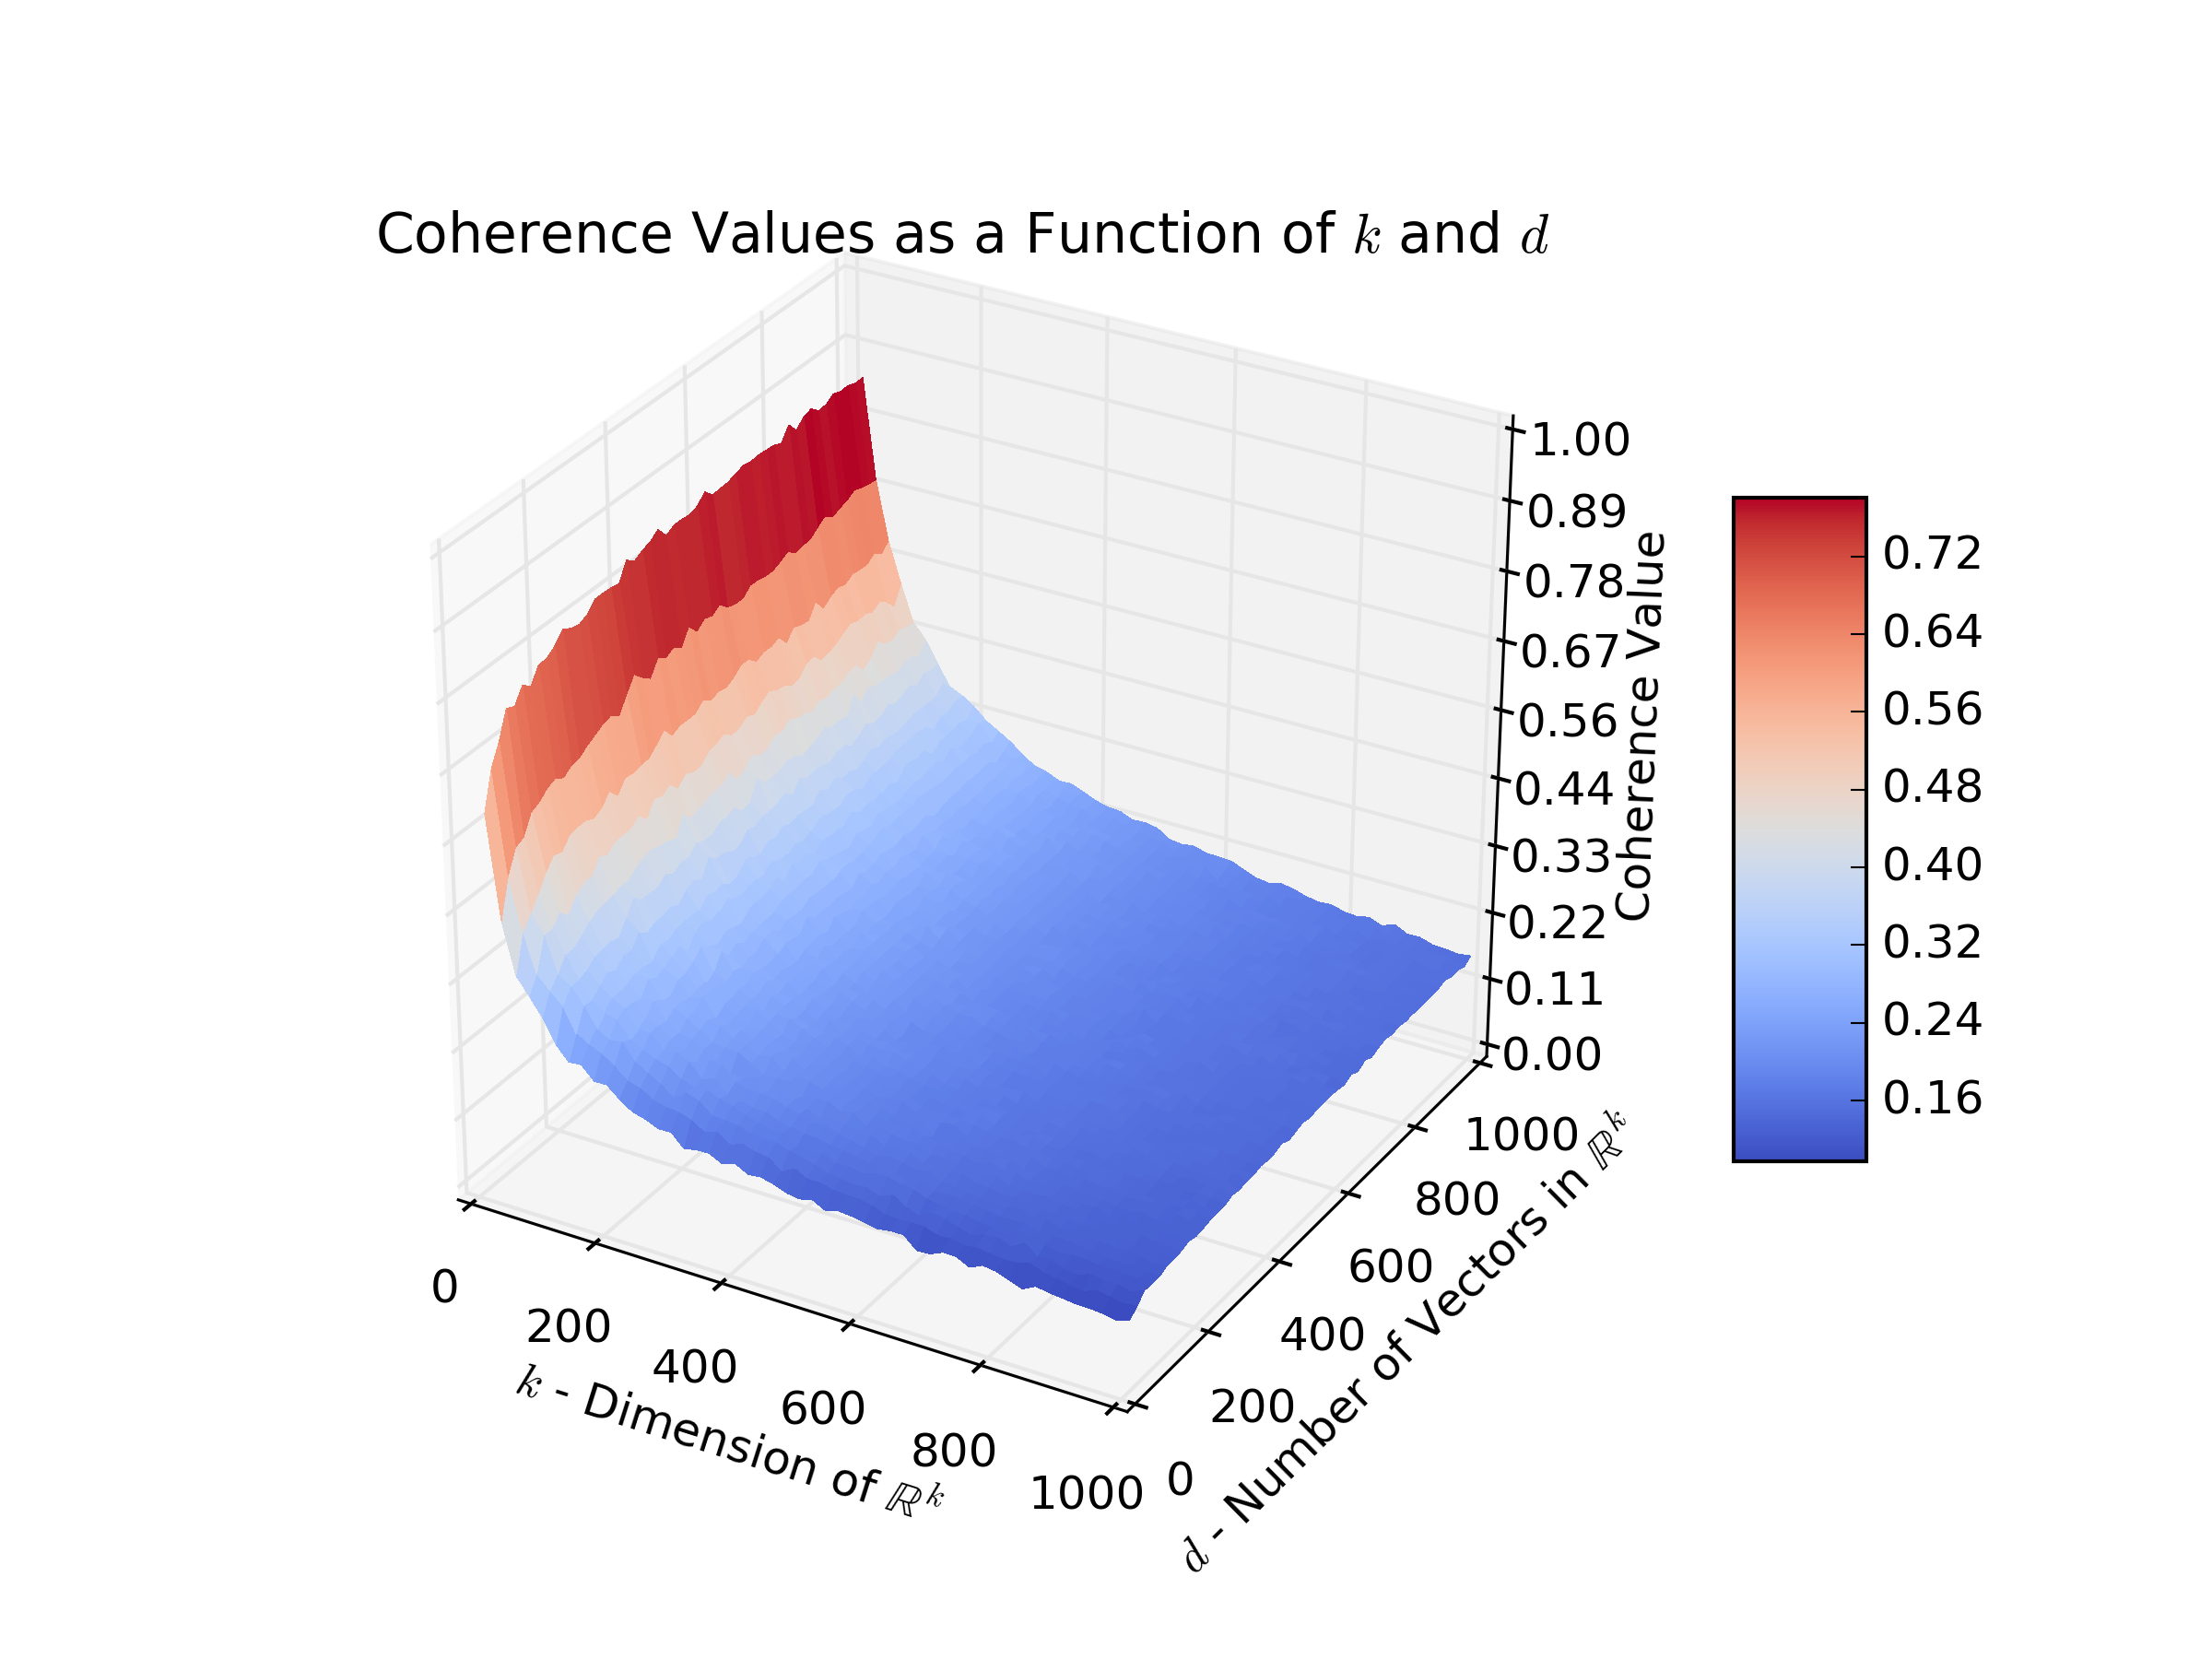
\includegraphics[width=\textwidth]{problem_3.png}
    \end{figure}
    The figure shows that coherence, in general, increases as the dimension decreases, and as the number of vectors increases.  This is intuitive since, as we saw from Homework 1 Problem 1, as the dimension decreases and/or the number of vectors increases, the probability that two vectors are close to orthogonal decreases.  Equivalently, the probability that two vectors are close to parallel increases.  If a matrix has two parallel columns, the coherence is $1$.
\end{proof}
    







%%%%%%%%%%%%%%%%%%%%%%%%%%%%%%%%%%%%%%
\problem{Problem 4}{Consider $y = Ax$, where $A$ is a $100 \times 400$ Gaussian random matrix and $x$ is a $s$-sparse vector of length $400$.  The locations of the non-zero entries of $x$ are chosen uniformly at random and the non-zero coefficients of $x$ are normal-distributed.  For $s = 1, 2, \dots, $ solve
\begin{align*}
    \min_z \norm{z}_1 \qquad \text{subject to } Az = y,
\end{align*}
(e.g.~using the toolbox CVX).  For each fixed $s$ repeat the experiment $10$ times.  Create a graph plotting $s$ versus the relative reconstruction error (averaged over the ten experiments for each $s$).  Starting with which value of $s$ approximately does $\ell_1$-minimization fail to recover $x$?}
\begin{proof}
    The following graph shows the mean $\ell^2$-norm errors of $10$ experiments at each $s$ for $s = 1, 2, \dots, 40$.  The non-zero entries of $x$ are normally distributed around $0$ with standard deviation of $1$.
    \begin{figure}[ht!]
        \centering
        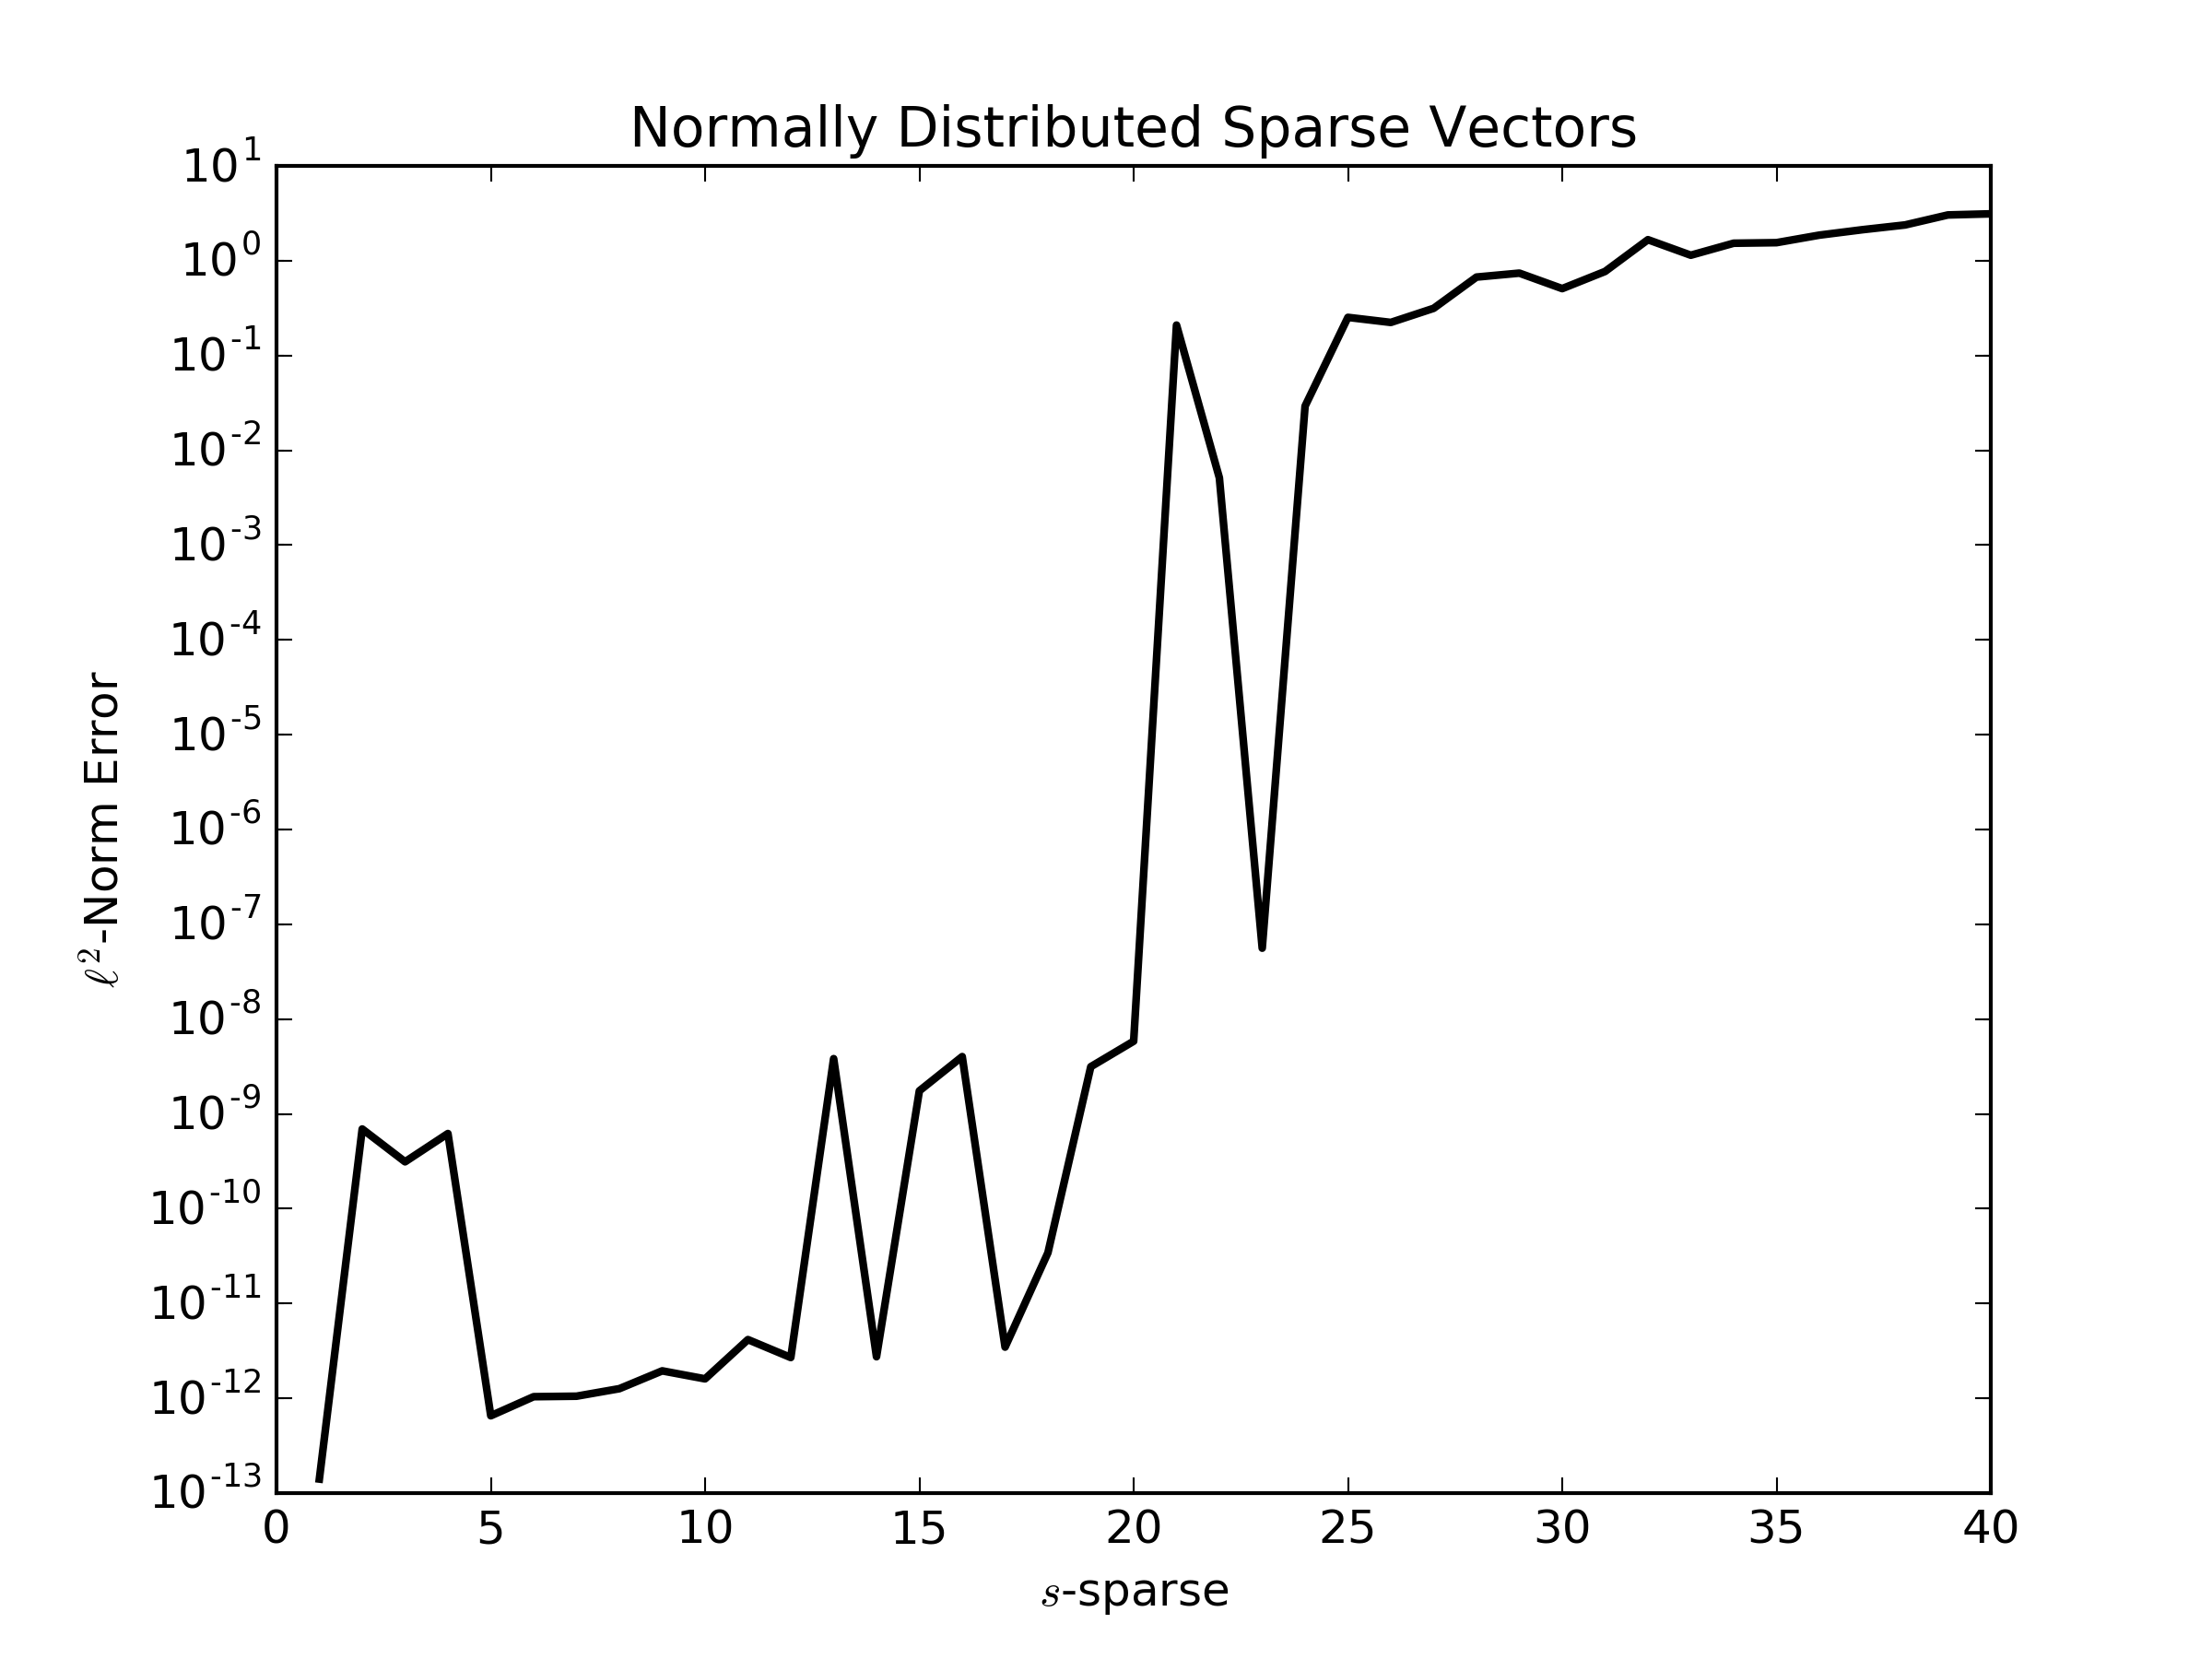
\includegraphics[width=\textwidth]{normally_distributed.png}
    \end{figure}
    In this experiment, this method failed for $s \geq 21$.
\end{proof}
    







%%%%%%%%%%%%%%%%%%%%%%%%%%%%%%%%%%%%%%
\problem{Problem 5}{Same setup as in Problem $4$, but now the non-zero entries of $x$ are non-negative.  Taking this information into account, we now solve
\begin{align*}
    \min_z \norm{z}_1 \qquad \text{subject to } Ax = y \text{ and } z \geq 0
\end{align*}
(here, $z \geq 0$ is meant entrywise, i.e., for each $k$, $z_k \geq 0$).  (The positivity constraint is easy to include in CVX).  Repeat the simulations as described in Problem 4.  Compare your findings to the results from your experiments of Problem 4 and try to quantify the difference regarding the range for $s$ for which recovery is still possible in this case.}
\begin{proof}
    The following graph shows the mean $\ell^2$-norm errors of $10$ experiments at each $s$ for $s = 1, 2, \dots, 40$.  The non-zero entries of $x$ are the absolute value of a normal distribution around $0$ with standard deviation of $1$.
    \begin{figure}[ht!]
        \centering
        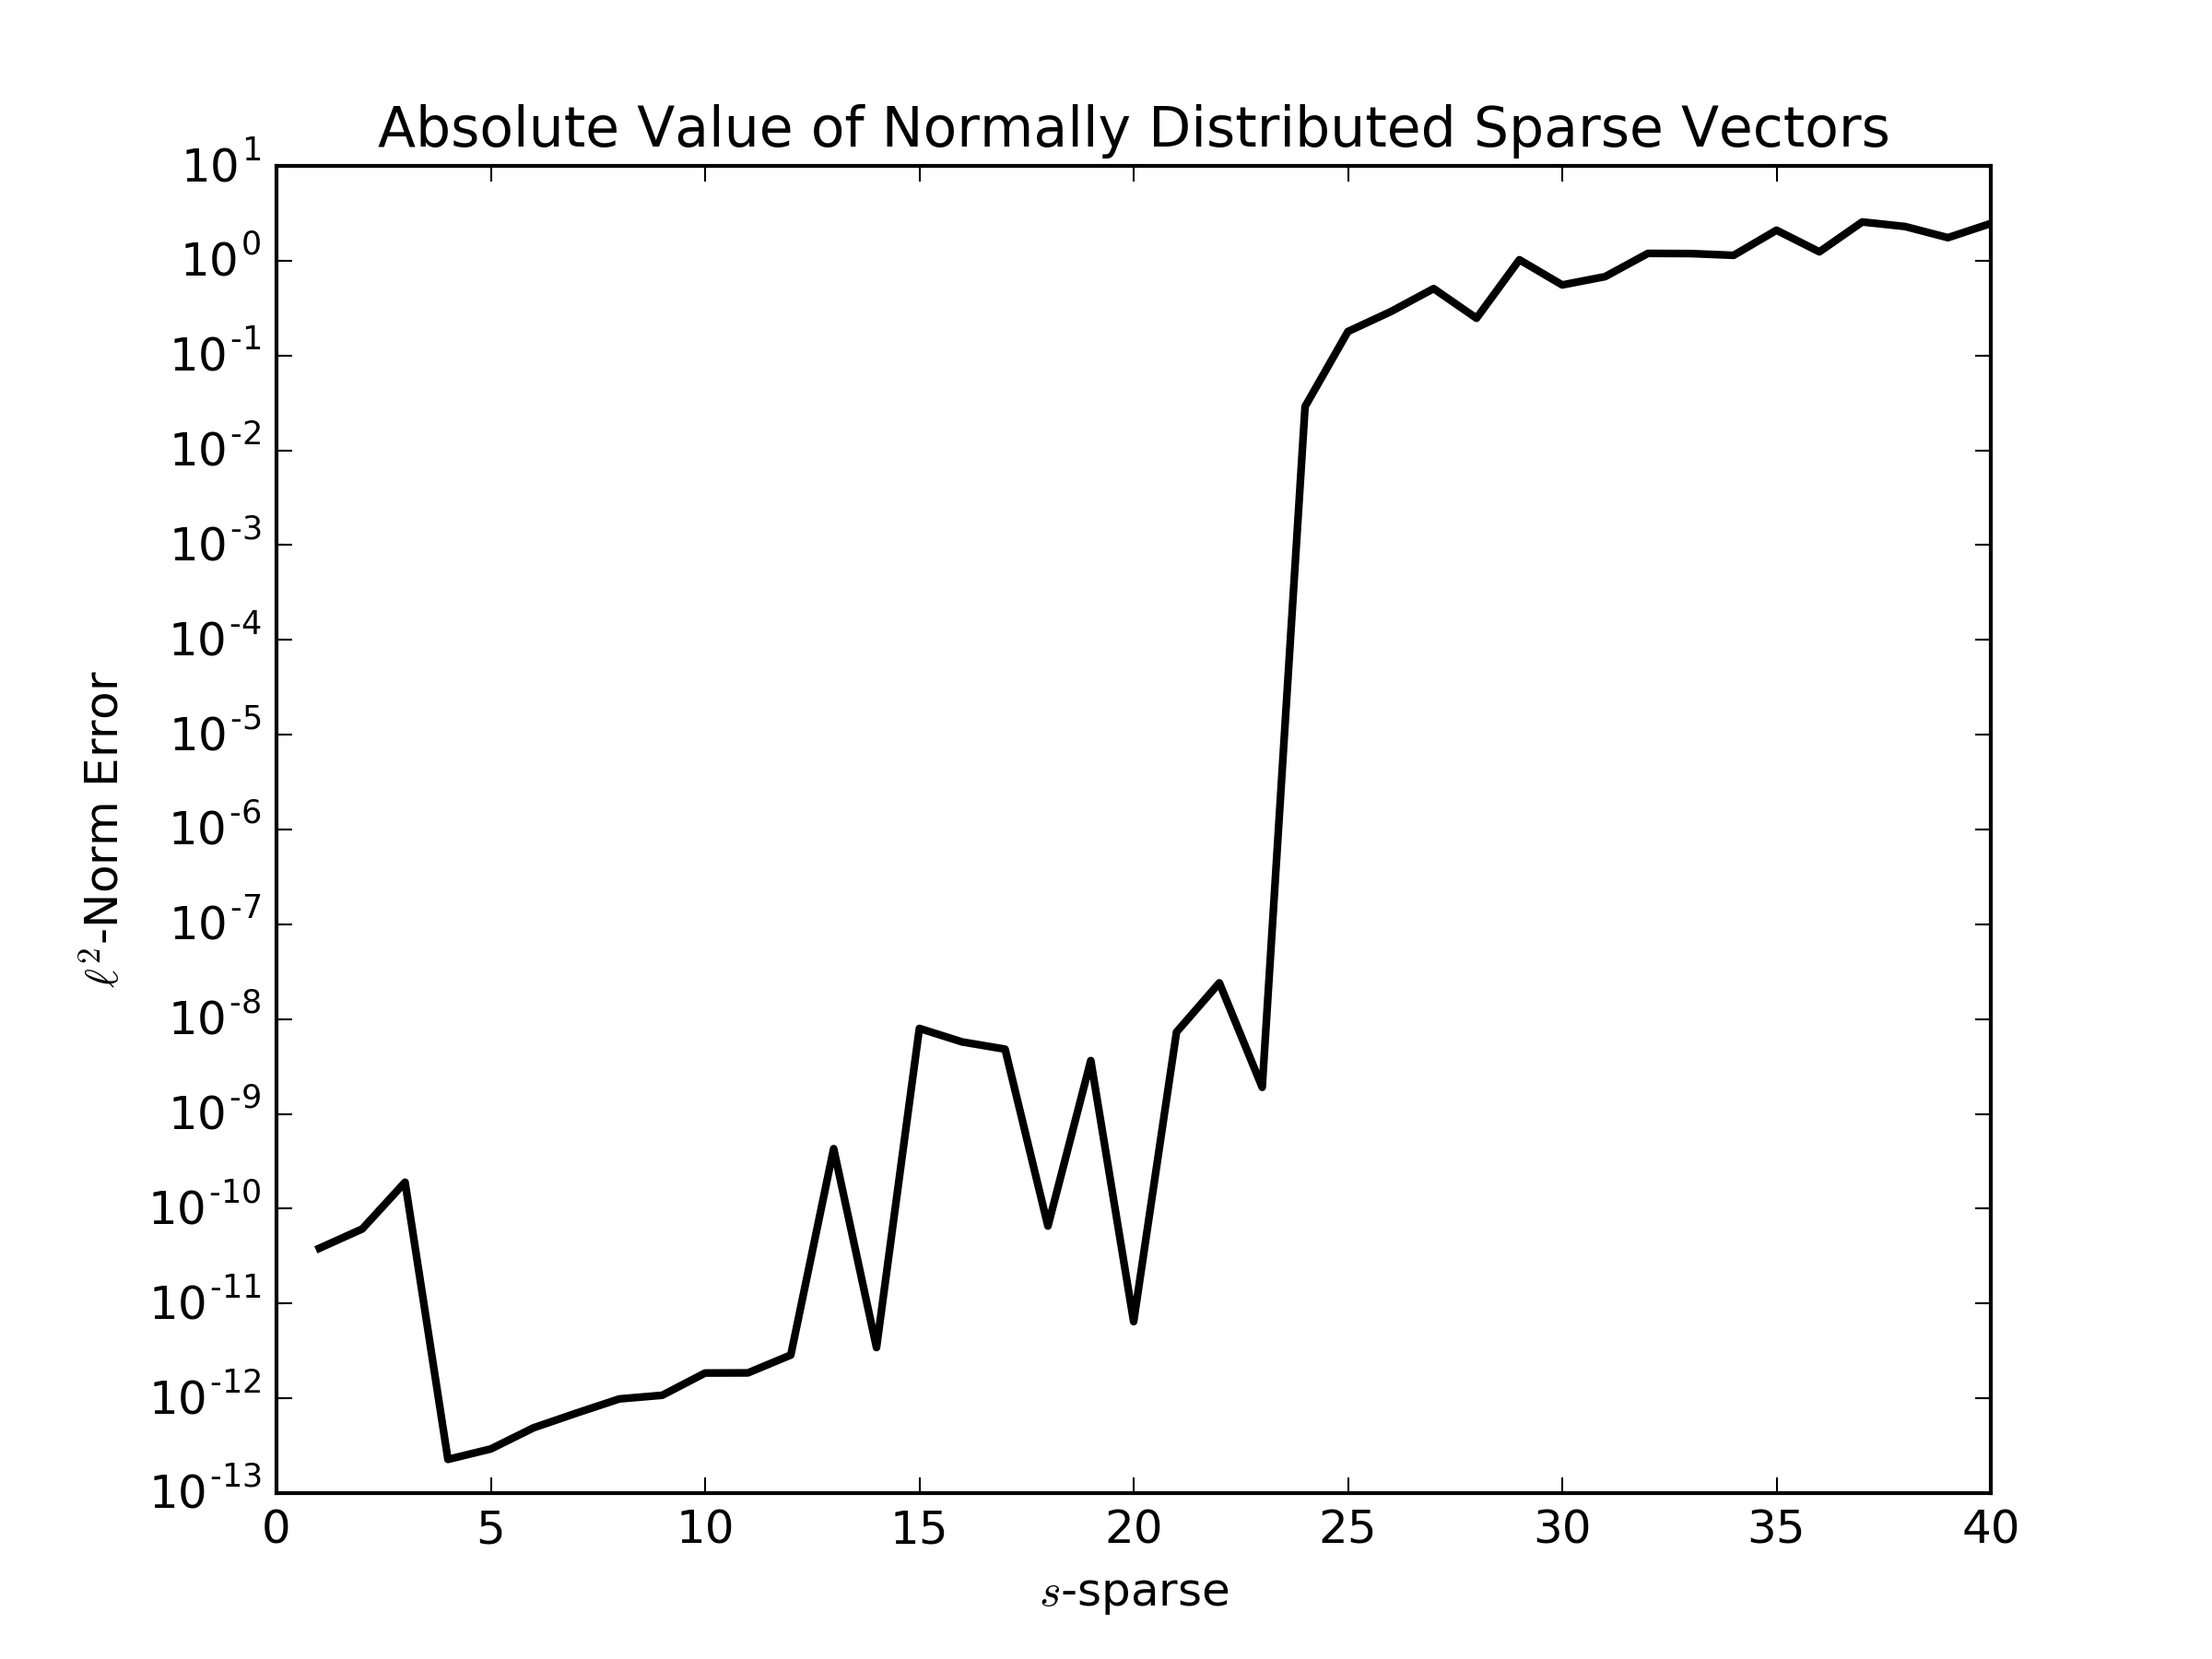
\includegraphics[width=\textwidth]{normally_distributed_nonnegative.png}
    \end{figure}
    In this experiment, this method failed for $s \geq 24$.
\end{proof}
    







\end{document}
